\documentclass[11pt,a4paper]{article}
\usepackage{amsmath}
\usepackage{amssymb}
\usepackage{graphicx}
\usepackage{subfigure}
\usepackage{float}
\usepackage{xeCJK}
\usepackage{geometry}
\geometry{left=2.0cm,right=2.0cm,top=2.0cm,bottom=2.0cm}

\usepackage{underscore}

\usepackage[T1]{fontenc}
\usepackage{xcolor}
\usepackage{lmodern}
\usepackage{listings}
\definecolor{mygreen}{rgb}{0,0.6,0}
\definecolor{mygray}{rgb}{0.5,0.5,0.5}
\definecolor{mymauve}{rgb}{0.58,0,0.82}

\lstset{
	basicstyle=\footnotesize,        % the size of the fonts that are used for the code
	breakatwhitespace=false,         % sets if automatic breaks should only happen at whitespace
	breaklines=false,                 % sets automatic line breaking
	captionpos=b,                    % sets the caption-position to bottom
	commentstyle=\color{mygreen},    % comment style
	extendedchars=true,              % lets you use non-ASCII characters; for 8-bits encodings only, does not work with UTF-8
	keepspaces=true,                 % keeps spaces in text, useful for keeping indentation of code (possibly needs columns=flexible)
	keywordstyle=\color{blue},       % keyword style
	language=[95]Fortran,                 % the language of the code
	numbers=left,                    % where to put the line-numbers; possible values are (none, left, right)
	numbersep=5pt,                   % how far the line-numbers are from the code
	numberstyle=\tiny\color{mygray}, % the style that is used for the line-numbers
	rulecolor=\color{black},         % if not set, the frame-color may be changed on line-breaks within not-black text (e.g. comments (green here))
	showspaces=false,                % show spaces everywhere adding particular underscores; it overrides 'showstringspaces'
	showstringspaces=false,          % underline spaces within strings only
	showtabs=false,                  % show tabs within strings adding particular underscores
	stepnumber=1,                    % the step between two line-numbers. If it's 1, each line will be numbered
	stringstyle=\color{mymauve},     % string literal style
	tabsize=4,                       % sets default tabsize to 2 spaces
	title=\lstname                   % show the filename of files
}


\title{P3DFFT库初始化}
\author{任广智}
\date{\today}


\begin{document}
	
\maketitle


实空间和谱空间的转换
\begin{equation}
	(N_x,\frac{N_y}{M_1},\frac{N_z}{M_2}) \sim (\frac{N_x+2}{2M_1},\frac{N_y}{M2},N_z) 
\end{equation}

转换到我们定义的变量即为
\begin{equation}
	(N_z,\frac{N_y}{M_2},\frac{N_x}{M_1}) \sim (\frac{N_z+2}{2M_2},\frac{N_y}{M1},N_x)
\end{equation}
所以,单进程下,当我们定义实空间网格数为(64,256,256)时,相应的谱空间网格数应该为(33,256,256)
为了方便比较,我们定义谱空间网格数为(64,256,256),则相应的实空间网格数为(126,256,256)。可以测试输出:
\begin{figure}[H]
	\centering
	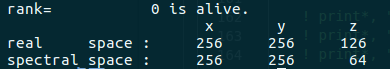
\includegraphics[width=0.5\textwidth]{./fig1.png}
	\caption{}
\end{figure}

那么考虑MPI并行化之后的情况,首先考虑2核的情况。假如系统中给出的并行方案是沿x方向并行,则预测实空间输出为(128,256,126),而谱空间输出为(256,128,64)。测试输出:
\begin{figure}[H]
	\centering
	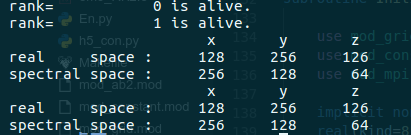
\includegraphics[width=0.5\textwidth]{./fig2.png}
	\caption{}
\end{figure}
可以看到两个进程的存在,而且网格划分符合预期。我这里是从谱空间开始的,即并行化方案根据(y-z)的网格来给出。所以这里两个进程实际上为谱空间中y方向上的网格划分,即(2)式中$M_1=2,M_2=1$,所以,当转换到实空间的时候,就变成了在x方向上的网格划分。这验证了(2)式的正确性。

进一步地,定义实空间中MPI二维并行化之后的网格数为(N_z,N_y_p,N_x_p),谱空间中并行化的方案为(K_z_p,K_y_p,N_x),我们可以通过8核运算来验证之前的结论。

\begin{figure}[H]
	\centering
	\subfigure[]{
		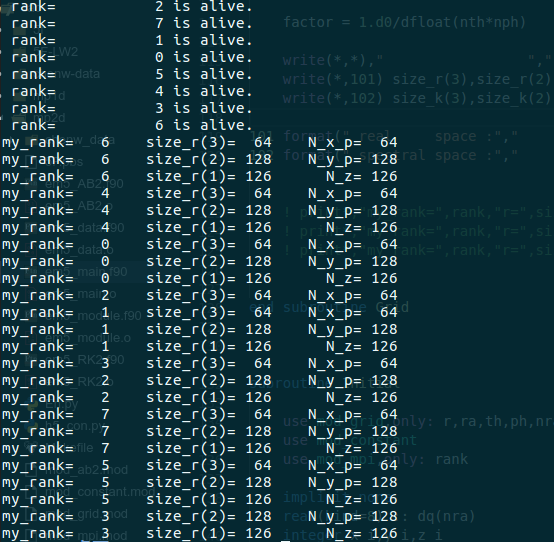
\includegraphics[width=0.4\textwidth]{./fig3.png} 
	}
	\subfigure[]{
		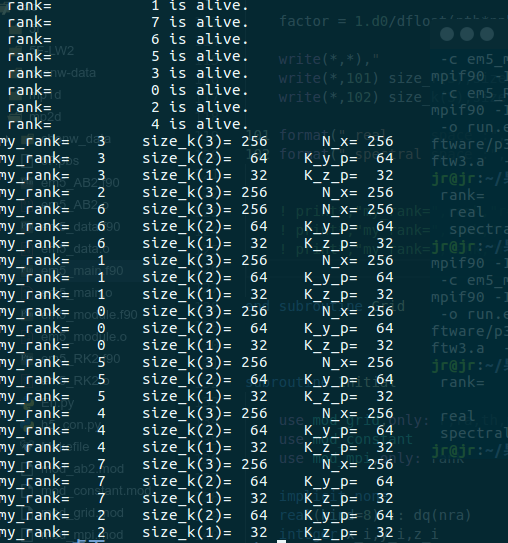
\includegraphics[width=0.4\textwidth]{./fig4.png}
	}
	\caption{}
\end{figure}
可以看出,实空间谱空间的网格划分均符合我们的预期。

需要注意的是,以上的例子都是无论在实空间还是谱空间中,经过划分的网格大小在每个进程当中都是一样的,当出现总网格数不能整除这个维度上的进程数的时候,P3DFFT库会自动采取另外的划分方案,即进程中的网格数不一定一致,使用时要注意。

所以,回到P3DFFT库的初始化上,初始如果在实空间采取2维MPI的并行方案,则dim_xy(0)为径向进程数,dim_xy(1)为极向进程数,则P3DFFT库的初始化应该为
\begin{lstlisting}
dim_p3d(0) = dim_xy(1)
dim_p3d(1) = dim_xy(0)

call P3DFFT_SETUP(MPI_comm_world, dim_p3d, nph, nth, nra, .true., memsize)
call P3DFFT_GET_DIMS(start_r, end_r, size_r, 1)
call P3DFFT_GET_DIMS(start_k, end_k, size_k, 2)
\end{lstlisting}
当在谱空间采用2维并行化方案时,则dim_yz代表极向和环向的进程数,则P3DFFT库初始化应该为:
\begin{lstlisting}
dim_p3d(0) = dim_yz(1)	! kz -> ny	M2
dim_p3d(1) = dim_yz(0)	! ky -> nx	M1

call P3DFFT_SETUP(MPI_comm_world, dim_p3d , nph, nth, nra, .true., memsize)
call P3DFFT_GET_DIMS(start_r, end_r, size_r, 1)
call P3DFFT_GET_DIMS(start_k, end_k, size_k, 2)
\end{lstlisting}


在上述两进程的例子中,如果我们使用了错误的初始化,即进程数在两个维度上给反的情况时,则上述分析不一定能成立,除非M1=M2。




\end{document}